\documentclass[openany,twoside, notitlepage,letterpaper,11pt]{book}

%%% These are the packages that are used
%used for custom page headers and page numbering
\usepackage{lipsum}
\usepackage{fancyhdr}
%adds TeX fonts from the American Mathematical Society.
\usepackage{amsfonts}
%Sets the bounds of the page margins
\usepackage[top=1in, bottom=1in, left=0.7in, right=.7in]{geometry}
%Various useful packages
\usepackage{amsmath,amssymb, amscd,amsbsy, amsthm, enumerate}
\usepackage{mdframed, titlesec, setspace,verbatim, multicol, caption}
\usepackage[unicode]{hyperref}
\usepackage{wasysym}
\usepackage{tikz, polynom}
\usepackage{xcolor}
\usepackage{etoolbox}
%enables the ability of including pages from a pdf.
\usepackage{pdfpages}
%enables drawings of circuit diagrams
\usepackage{circuitikz}

%enables changing the bibliography name
\usepackage[nottoc,notlof,notlot]{tocbibind}

%enables indexing
\usepackage{makeidx} 
%makes the index size footnote
\usepackage[font=footnotesize, columns=3]{idxlayout}

%Adds extra symbols
\usepackage{mathrsfs, upgreek}

%Allows for tables with cells that span multiple rows and columns
\usepackage{multirow}



%This is where settings for the latex file are stored.
%%Version Number
\newcommand{\Version}{2.000 beta}
%%Version

%%% Page formatting
%\setlength{\headsep}{30pt}
\setlength{\parindent}{25pt}
\setlength{\textheight}{9in}

%Rename the bibliography to References.
\renewcommand\bibname{References}


%%% Header and Footer Info
\pagestyle{fancy}
\fancyhead[LO]{\small {\textbf{Antonius' Handbook -- Version \Version}}}
\fancyhead[RE]{\small {\textbf{Antonius' Handbook -- Version \Version}}}
\fancyhead[C]{}
\fancyhead[RO]{\small \thepage}
\fancyhead[LE]{\small \thepage}
\fancyfoot[L]{}
\fancyfoot[C]{}
\fancyfoot[R]{}


\patchcmd{\chapter}{plain}{empty}{}{}
\titleformat{\chapter}[display]
{\normalfont\huge\bfseries}{}{0pt}{\Huge}
\titlespacing*{\chapter} {0pt}{-50pt}{10pt}

%This is where custom definitions and variables are defined and stored.
\newcommand{\andspace}[1]{\hspace{#1}\textrm{and}\hspace{#1}}

\numberwithin{equation}{section}
\setlength{\columnsep}{.5cm}
\setlength{\columnseprule}{1pt}
\def\columnseprulecolor{\color{black}}

\newcommand{\abs}[1]{\left| #1 \right|}
\newcommand{\inner}[1]{\langle #1 \rangle}
\newcommand{\norm}[1]{\left\lVert#1\right\rVert}
\newcommand{\spanvect}{\textnormal{span}}
\newcommand{\union}{\cup}
\newcommand{\Union}{\bigcup}

%create a section without making the section title.
\newcommand\invisiblesection[1]{%
	\refstepcounter{section}%
	\addcontentsline{toc}{section}{\protect\numberline{\thesection}#1}%
	\sectionmark{#1}}

%Makes a chapter with no title
\makeatletter
\newcommand{\unchapter}[1]{%
	\begingroup
	\let\@makechapterhead\@gobble % make \@makechapterhead do nothing
	\chapter{#1}
	\endgroup
}
\makeatother


%%% This defines the solution environment for you to write your solutions
\newenvironment{soln}
{\let\oldqedsymbol=\qedsymbol
	\renewcommand{\qedsymbol}{$ $}
	\begin{proof}[\bfseries\upshape \color{blue}Derivation]\color{blue}}
	{\end{proof}
	\renewcommand{\qedsymbol}{\oldqedsymbol}}

\newenvironment{note}
{\let\oldqedsymbol=\qedsymbol
	\renewcommand{\qedsymbol}{$ $}
	\begin{proof}[\bfseries\upshape \color{red}Note]\color{red}}
	{\end{proof}
	\renewcommand{\qedsymbol}{\oldqedsymbol}}


%theorem
\newcounter{theo}[section] \setcounter{theo}{0}
\renewcommand{\thetheo}{\arabic{section}.\arabic{theo}}
\newenvironment{theo}[2][]{%
	\refstepcounter{theo}%
	\ifstrempty{#1}%
	{\mdfsetup{%
			frametitle={%
				\tikz[baseline=(current bounding box.east),outer sep=0pt]
				\node[anchor=east,rectangle,fill=blue!20]
				{\strut Theorem~\thetheo};}}
	}%
	{\mdfsetup{%
			frametitle={%
				\tikz[baseline=(current bounding box.east),outer sep=0pt]
				\node[anchor=east,rectangle,fill=blue!20]
				{\strut Theorem~\thetheo:~#1};}}%
	}%
	\mdfsetup{innertopmargin=10pt,linecolor=blue!20,%
		linewidth=2pt,topline=true,%
		frametitleaboveskip=\dimexpr-\ht\strutbox\relax
	}
	\begin{mdframed}[]\relax%
		\label{#2}}{\end{mdframed}}
%%%%%%%%%%%%%%%%%%%%%%%%%%%%%%
%Lemma
\newcounter{lemm}[section] \setcounter{lemm}{0}
\renewcommand{\thelemm}{\arabic{chapter}.\arabic{lemm}}
\newenvironment{lemm}[2][]{%
	\refstepcounter{lemm}%
	\ifstrempty{#1}%
	{\mdfsetup{%
			frametitle={%
				\tikz[baseline=(current bounding box.east),outer sep=0pt]
				\node[anchor=east,rectangle,fill=green!20]
				{\strut Lemma~\thelem};}}
	}%
	{\mdfsetup{%
			frametitle={%
				\tikz[baseline=(current bounding box.east),outer sep=0pt]
				\node[anchor=east,rectangle,fill=green!20]
				{\strut Lemma~\thelem:~#1};}}%
	}%
	\mdfsetup{innertopmargin=10pt,linecolor=green!20,%
		linewidth=2pt,topline=true,%
		frametitleaboveskip=\dimexpr-\ht\strutbox\relax
	}
	\begin{mdframed}[]\relax%
		\label{#2}}{\end{mdframed}}
%%%%%%%%%%%%%%%%%%%%%%%%%%%%%%
%Proof
\newcounter{prf}[section]\setcounter{prf}{0}
\renewcommand{\theprf}{\arabic{chapter}.\arabic{prf}}
\newenvironment{prf}[2][]{%
	\refstepcounter{prf}%
	\ifstrempty{#1}%
	{\mdfsetup{%
			frametitle={%
				\tikz[baseline=(current bounding box.east),outer sep=0pt]
				\node[anchor=east,rectangle,fill=red!20]
				{\strut Proof~\theprf};}}
	}%
	{\mdfsetup{%
			frametitle={%
				\tikz[baseline=(current bounding box.east),outer sep=0pt]
				\node[anchor=east,rectangle,fill=red!20]
				{\strut Proof~\theprf:~#1};}}%
	}%
	\mdfsetup{innertopmargin=10pt,linecolor=red!20,%
		linewidth=2pt,topline=true,%
		frametitleaboveskip=\dimexpr-\ht\strutbox\relax
	}
	\begin{mdframed}[]\relax%
		\label{#2}}{\qed\end{mdframed}}
%%%%%%%%%%%%%%%%%%%%%%%%%%%%%%
%Definition
\newcounter{defn}[section] \setcounter{defn}{0}
\renewcommand{\thedefn}{\arabic{chapter}.\arabic{defn}}
\newenvironment{defn}[2][]{%
	\refstepcounter{defn}%
	\ifstrempty{#1}%
	{\mdfsetup{%
			frametitle={%
				\tikz[baseline=(current bounding box.east),outer sep=0pt]
				\node[anchor=east,rectangle,fill=gray!20]
				{\strut Definition~\thedefn};}}
	}%
	{\mdfsetup{%
			frametitle={%
				\tikz[baseline=(current bounding box.east),outer sep=0pt]
				\node[anchor=east,rectangle,fill=gray!20]
				{\strut Definition~\thedefn:~#1};}}%
	}%
	\mdfsetup{innertopmargin=10pt,linecolor=gray!20,%
		linewidth=2pt,topline=true,%
		frametitleaboveskip=\dimexpr-\ht\strutbox\relax
	}
	\begin{mdframed}[nobreak=true]\relax%
		\label{#2}}{\end{mdframed}}
%Fancy Box
\newcounter{fancybox}[section] \setcounter{fancybox}{0}
\renewcommand{\thefancybox}{\arabic{chapter}.\arabic{fancybox}}
\newenvironment{fancybox}[2][]{%
	\refstepcounter{fancybox}%
	\ifstrempty{#1}%
	{\mdfsetup{%
			frametitle={%
				\tikz[baseline=(current bounding box.east),outer sep=0pt]
				\node[anchor=east,rectangle,fill=orange!20]
				{\strut ~\thefancybox};}}
	}%
	{\mdfsetup{%
			frametitle={%
				\tikz[baseline=(current bounding box.east),outer sep=0pt]
				\node[anchor=east,rectangle,fill=orange!20]
				{\strut ~\thefancybox:~#1};}}%
	}%
	\mdfsetup{innertopmargin=10pt,linecolor=orange!20,%
		linewidth=2pt,topline=true,%
		frametitleaboveskip=\dimexpr-\ht\strutbox\relax
	}
	\begin{mdframed}[]\relax%
		\label{#2}}{\end{mdframed}}

%creates the title page
\title{
\includegraphics[scale=.2]{./Images/Covers/AH2.png}
	\\ \vspace{1.5cm} Useful Formulas, Constants, Units and Definitions \\ Volume II - Programmers Paradise \\ Version \Version}
\date{}
\author{Compiled by: Antonius William Torode\\ Natural Science Department: Michigan State University \\ Written in: \LaTeX}

\makeindex
%\addcontentsline{toc}{chapter}{Index}


%%% Document Starts now
\begin{document}

%Begin the front matter.
\frontmatter
%Begins title page.
\maketitle
\thispagestyle{empty}
\pagestyle{empty}
\begin{center}
	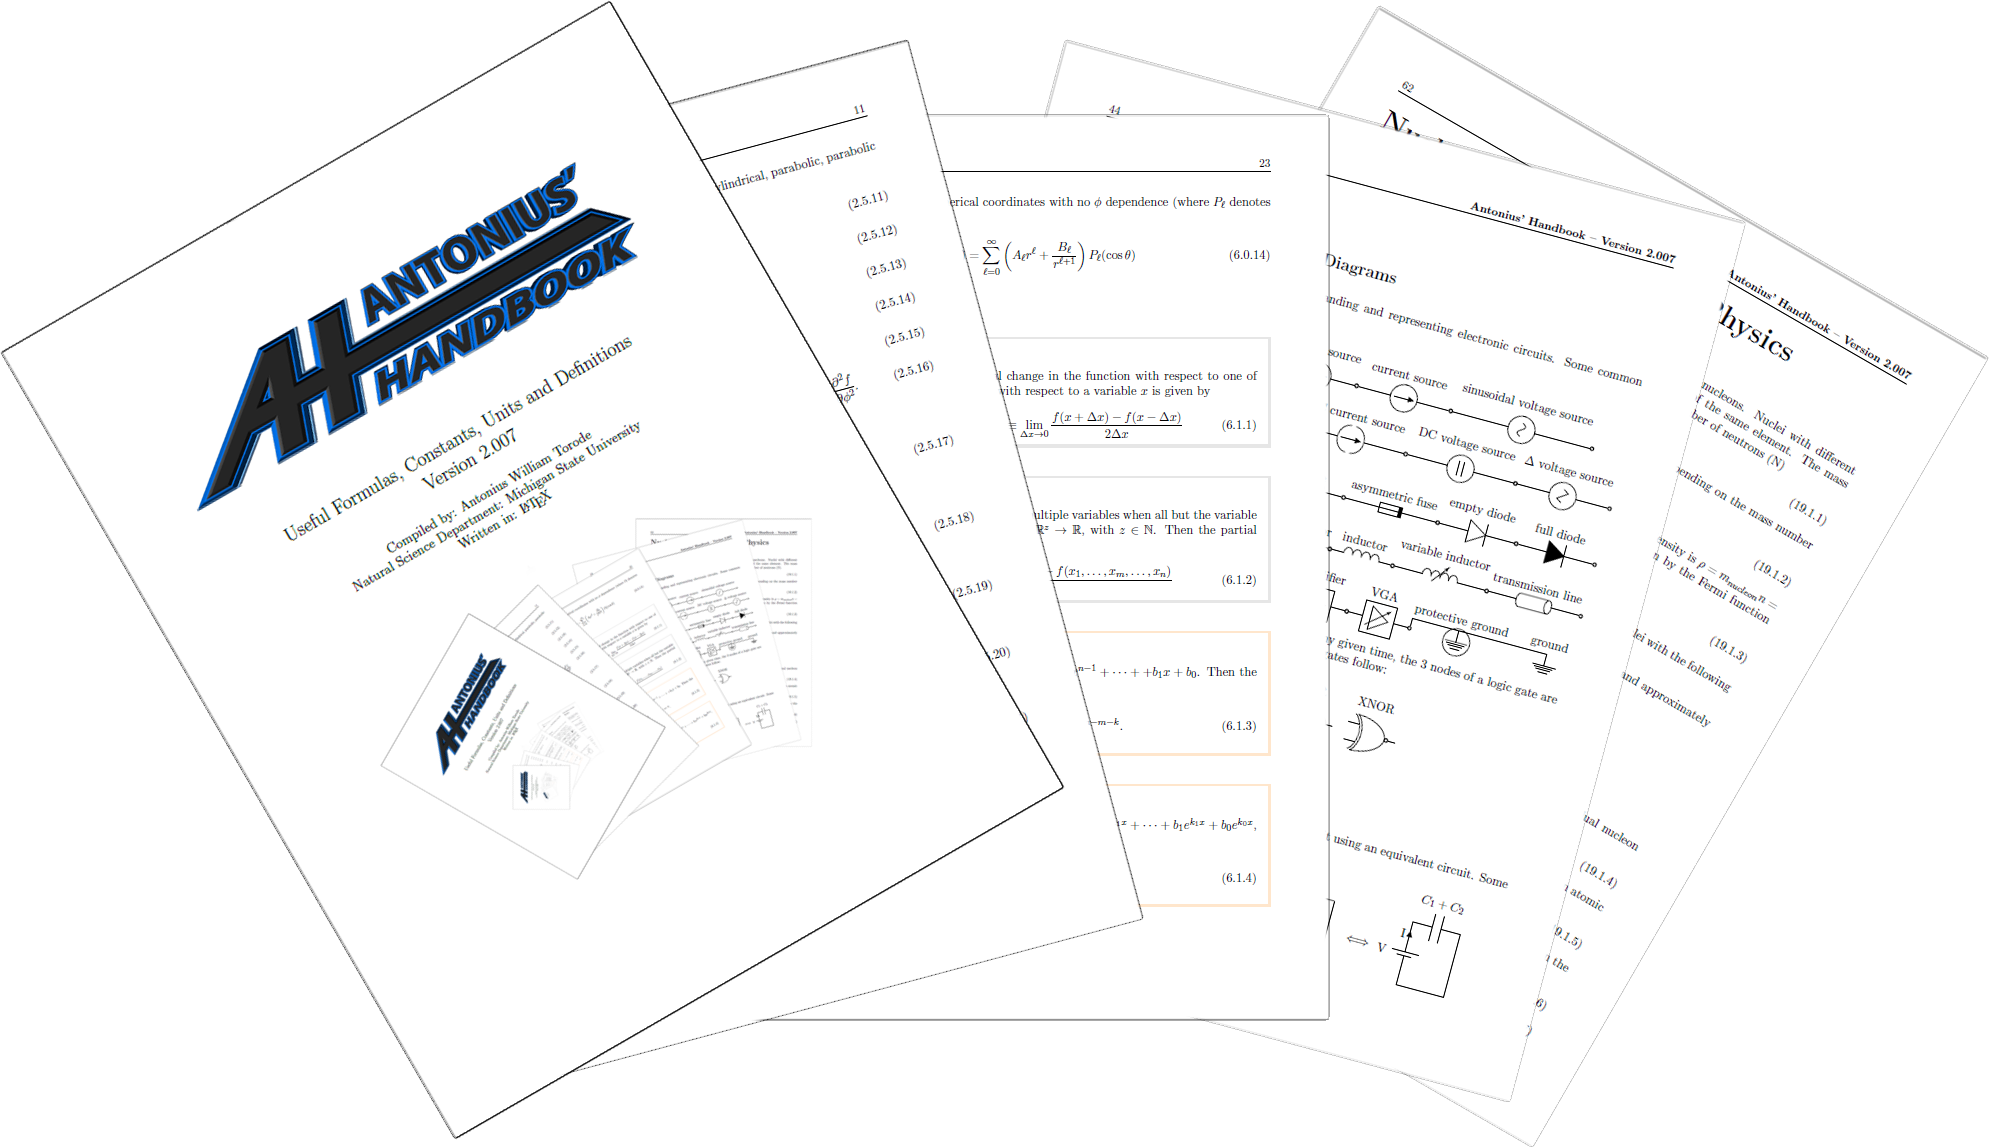
\includegraphics[scale=1.8]{./Images/Covers/background_tunnel.png}
\end{center}

%Copywrite page
\pagestyle{empty}
%% copyrightpage
\begingroup
\footnotesize
\parindent 0pt
\parskip \baselineskip
\textcopyright{} 2016 Antonius Torode \\
All rights reserved.

This work may be distributed and/or modified under the conditions of the Antonius' Handbook License.

The original maintainer of this work is: Antonius Torode.

The current maintainer of this work is: Antonius Torode.

Published by Antonius Torode. 

Hosted at: https://msu.edu/{\raise.17ex\hbox{$\scriptstyle\sim$}}torodean/AHandbook.html

Github Repository: https://github.com/torodean/Antonius-Handbook

\begin{center}
\begin{tabular}{ll}
First Personal Release (Version 0.000): & January 2016 \\
First Public Release (Version 1.000): &  July 2016 \\
Most Current Revision Date (Version 2.000+): & \today 
\end{tabular}
\end{center}

\vfill

Torode, A.\\
\hspace*{2em} Michigan State University -- \\
\hspace*{1em} Department of Physics \& Astronomy. \\
\hspace*{2em} 2016, Student. \\
\hspace*{2em} Version: \Version \\
\hspace*{2em} Includes References \\
\hspace*{2em} ISBN: NONE



\endgroup
\clearpage

%Preface page
\begin{center}
	\textbf{Preface}
\end{center}

This document is a compilation of useful formulas, definitions, constants, and general information used throughout my own schooling as a reference while furthering education. It's purpose is to provide a complete 'encyclopedia' per say of various mathematical and significant ideas used often. The idea and motivation behind it is to be a quick reference providing easily accessible access to necessary information for either double checking or recalling proper formula for use in various situations due to my own shortcomings in matters of memorization. All the material in this document was either directly copied from one of the references listed at the end or derived from scratch. On occasion typos may exist due to human error but will be corrected when discovered.
	
The version number is updated every time the document is distributed, printed, or referred to. This ensures that there is no two copies with different information and similar version numbers. The latest update date is automatically set to the current date each time the document is edited. Please refrain from distributing this handbook without permission from the original author/compiler. As of version 1.035 this book is formatted for printing.

\begin{center}
	\textbf{Courses Covered In This Book}
\end{center}

This document encompasses a large portion of formula used throughout specific courses at Michigan state University. The courses which have information pertaining to something in this book are more than just listed below; however, below is a list of classes that the author took whilst compiling the information in this book. All course numbers correspond to Michigan State University courses at the time of adding them. 

\begin{multicols}{2}
\begin{itemize}
	\item AST 207/208/304: Astrophysics I/II/III
	\item PHY 215: Thermodynamics \& Modern Physics
	\item MTH 310: Abstract Algebra/Number Theory
	\item PHY 321: Classical Mechanics I
	\item PHY 410: Thermal \& Statistical Physics
	\item PHY 415: Methods Of Theoretical Physics
	\item PHY 440: Electronics
	\item PHY 471/472: Quantum Physics I/II
	\item PHY 481/482: Electricity and Magnetism I/II
	\item PHY 492: Introduction to Nuclear Physics
\end{itemize} 
\end{multicols}

The information in this book is in no way limited to the material used within the courses above. They serve as a simple guideline to what you will find within this document. For more information about this book or details about how to obtain your own copy please visit:
\begin{center}
	https://msu.edu/{\raise.17ex\hbox{$\scriptstyle\sim$}}torodean/AHandbook.html
\end{center}
\begin{center}
	\textbf{Disclaimer}
\end{center}

This book contains formulas, definitions, and theorems that by nature are very precise. Due to this, some of the material in this book was taken directly from other sources such as but not limited to Wolfram Mathworld. This is only such in cases where a change in wording could cause ambiguities or loss of information quality.  Following this, all sources used are listed in the references section.

%Begins blank page.
\thispagestyle{empty}
\newpage
\vspace*{\stretch{1}}
\begin{center}
	\textit{This page intentionally left blank.\\ (Yes, this is a contradiction.)}
\end{center}
\vspace*{\stretch{1}}

%Begins table of contents
\tableofcontents


%Begin the mainmatter.
\setlength{\parindent}{0pt}
\mainmatter
\pagestyle{fancy}
\chapter{Linux}
\thispagestyle{fancy}
\lstset{language=Bash, style=bash}

\section{System Related Commands\index{System Related Commands}}

Retreive information and valid arguments for a command.
\begin{lstlisting}
COMMAND --help   # COMMAND must be a valid command such as cd, ls, etc...
\end{lstlisting}

Changing directory via terminal
\begin{lstlisting}
cd /directory # Changes the directory to the subdirectory /directory
cd ..         # Goes back one directory
\end{lstlisting}

How to display the processes that are currently running.
\begin{lstlisting}
ps aux
\end{lstlisting}

To search the results of a command for a string of characters one can use the grep command. For example:
\begin{lstlisting}
ps aux | grep "firefox"
\end{lstlisting}

Restore power/battery icon if it disappears.
\begin{lstlisting}
/usr/lib/x86_64-linux-gnu/indicator-power/indicator-power-service &disown 
\end{lstlisting}

Restore volume icon/control button if it disappears.
\begin{lstlisting}
gsettings set com.canonical.indicator.sound visible true
\end{lstlisting}

Reset wifi services in case the connection gets lost.
\begin{lstlisting}
sudo systemctl restart network-manager.service
\end{lstlisting}

Turn off LCD display.
\begin{lstlisting}
xset dpms force off //turns off display.
\end{lstlisting}

Change or view the host name of a computer with the hostname file.
\begin{lstlisting}
sudo nano /etc/hostname # Opens this file using nano for editing.
hostname                # Command to see what the current hostname is.
\end{lstlisting}

Make a file executable and execute a file
\begin{lstlisting}
chmod a+x /location/of/FILE # Makes a file executable
./FILE                      # Executes a file.
\end{lstlisting}

\section{Files and Storage}

Copy a file or directory to a different linux computer
\begin{lstlisting}
#To copy a file.
scp <File Path> username@computer:"<path to copy to>"

#To copy a directory.
scp -r <File Path> username@computer:"<path to copy to>"
\end{lstlisting}

Show information about the file system on which each FILE resides, or all file systems by default.
\begin{lstlisting}
df 
\end{lstlisting}

List information about File(s) (in the current directory by default).
\begin{lstlisting}
ls        # list all items in a directory
ls -1     # list all items in a directory (one item per line)
ls -lh    # list all items in a directory with size, owner, and date modified
\end{lstlisting}

List all of the block devices (hence partitions) detected by the machine
\begin{lstlisting}
lsblk
\end{lstlisting}

Mount and unmount a partition
\begin{lstlisting}
sudo mount <DEVICE TO MOUNT> <MOUNT POINT>
sudo mount /dev/sdb1/ /mnt/      #example of mounting
sudo umount <DEVICE TO MOUNT> <MOUNT POINT>
sudo umount /dev/sdb1/ /mnt/      #example of mounting
\end{lstlisting}

\section{Users and Groups}

Create a new user
\begin{lstlisting}
sudo useradd [options] <USERNAME>             #Creates a user
sudo useradd -e 2016-02-05 <NAME>             #Creates a user that expites on a day.
sudo useradd <USERNAME> -G <GROUPNAME>        #Adds a user to a group upon creation.
useradd --help                                #See full useradd options.
\end{lstlisting}

Change a users password
\begin{lstlisting}
passwd <USERNAME>
\end{lstlisting}

Change the user in terminal
\begin{lstlisting}
su - <USERNAME>
\end{lstlisting}

Add a user to the sudoers group
\begin{lstlisting}
usermod -aG sudo <USERNAME>
\end{lstlisting}













\section{Networking\index{Networking}}

View IP configuration information
\begin{lstlisting}
ifconfig
\end{lstlisting}

Enable/Disable IPv6
\begin{lstlisting}
#Use these two commands to disable IPv6
sudo sysctl -w net.ipv6.conf.all.disable_ipv6=1
sudo sysctl -w net.ipv6.conf.default.disable_ipv6=1

#Use these two commands to re-enable IPv6
sudo sysctl -w net.ipv6.conf.all.disable_ipv6=0
sudo sysctl -w net.ipv6.conf.default.disable_ipv6=0
\end{lstlisting}

\newpage
\chapter{C}
\thispagestyle{fancy}

\newpage
\chapter{C++}
\thispagestyle{fancy}
\lstset{language=C++, style=cpp}

\section{Basic Input and Output\index{Input and Output}}
To output text via a terminal you can use:
\begin{lstlisting}
std::string text = "Hello World!";
std::cout << text << std::endl; //std::endl is equivalent to the new-line character.
\end{lstlisting}

To get input as a user in the type of a std::string, you can use:
\begin{lstlisting}
std::string input = "";
std::cout << "Enter some text: ";
std::getline(std::cin, input);
\end{lstlisting}

\subsection{Simulate Key Strokes (Windows Only)\index{Simulate Key Strokes}}

First the correct files must be included and an event must be setup.
\begin{lstlisting}
#define WINVER 0x0500
#include <windows.h> 

INPUT ip;

ip.type = INPUT_KEYBOARD; // Set up a generic keyboard event.    
ip.ki.wScan = 0; // hardware scan code for key                                   
ip.ki.time = 0;
ip.ki.dwExtraInfo = 0;
\end{lstlisting}

After this, functions can be setup to simulate various keys based on the specific key codes, two examples of such are
\begin{lstlisting}
void space(){ 
	// Press the "space" key.  
	ip.ki.wVk = VK_SPACE; // virtual-key code for the "space" key.                                                                                
	ip.ki.dwFlags = 0; // 0 for key press                                                                                                        
	SendInput(1, &ip, sizeof(INPUT));
	
	// Release the "space" key                                                                                                                   
	ip.ki.wVk = VK_SPACE; // virtual-key code for the "space" key.                                                                                
	ip.ki.dwFlags = KEYEVENTF_KEYUP; // KEYEVENTF_KEYUP for key release                                                                          
	SendInput(1, &ip, sizeof(INPUT));
	Sleep(50);
}

void one(){ 
	// Press the "1" key.    
	ip.ki.wVk = 0x31; // virtual-key code for the "1" key.                                          
	ip.ki.dwFlags = 0; // 0 for key press                                                                                                        
	SendInput(1, &ip, sizeof(INPUT));
	
	// Release the "1" key.                                                                                                                    
	ip.ki.wVk = 0x31; // virtual-key code for the "1" key.                                                                                      
	ip.ki.dwFlags = KEYEVENTF_KEYUP; // KEYEVENTF_KEYUP for key release.                                                                          
	SendInput(1, \&ip, sizeof(INPUT));
	Sleep(50);
}
\end{lstlisting}

A similar method can be used to simulate mouse clicks. And example for left click follows
\begin{lstlisting}
void leftclick(){
	INPUT ip={0};
	// left down                                                                                                                                   
	ip.type = INPUT_MOUSE;
	ip.mi.dwFlags = MOUSEEVENTF_LEFTDOWN;
	SendInput(1,&Input,sizeof(INPUT));
	
	// left up                                                                                                                                     
	ZeroMemory(&Input,sizeof(INPUT));
	ip.type = INPUT_MOUSE;
	ip.mi.dwFlags = MOUSEEVENTF_LEFTUP;
	SendInput(1,&Input,sizeof(INPUT));
	Sleep(50);
}
\end{lstlisting}


\section{Variable Types\index{Variable Types}}

Creating and using a vector\index{Vector}.
\begin{lstlisting}
#include <vector>

int size1 = 5;
int size2 = 6;

//Creates a vector named V1 containing int's with a size of 5 and sets each element to 0. 
std::vector<int> V1(size1, 0); 

//Creates a 2-D vector (vector containing vectors) of size 5x6 named V2 containing doubles;
std::vector< std::vector<double>> V2(size1, std::vector<double>(size2, 0)); 

V1[0] = 8; //Sets the first element in V1 to 8.

V2[0][3] = 3.1415; //Sets the 4th element in the first row of V2 to 3.1415.

\end{lstlisting}


\subsection{Converting Between Types\index{Converting Between Types}}

\subsection*{std::string to int\index{std::string to int}}
To convert a string to an integer you can use:
\begin{lstlisting}
std::string text = "31415";
int number = std::stoi(text);
\end{lstlisting}

\section{Mathematical Commands}

\subsection*{Prime Number\index{Prime Number}}
A simple brute for method to determines if a number of type long is prime or not.
\begin{lstlisting}
bool isPrime(long num) {  
	int c = 0;   //c is a counter for how many numbers can divide evenly into num
	if (num == 0 || num == 1 || num == 4) {
		return false;
	}
	for (long i = 1; i <= ((num + 1) / 2); i++) {
		if (c < 2) {
			if (num % i == 0) {
				c++;
			}
		} else {
			return false;
		}
	}
	return true;
}
\end{lstlisting}

\section{System Commands\index{System Commands}}

\subsection*{Sleep\index{Sleep}}
Make the thread sleep for some amount of time using the std::chrono to determine the duration \cite{cpp:chrono}.
\begin{lstlisting}
#include <thread>
#include <chrono>

std::this_thread::sleep_for(std::chrono::milliseconds(50)); //Makes the system sleep for 50 milliseconds.

std::this_thread::sleep_for(std::chrono::seconds(50)); //Makes the system sleep for 50 seconds.
\end{lstlisting}

On a Windows specific program this can be simplified by including the windows.h header
\begin{lstlisting}
#include <windows.h>

Sleep(50); //Makes the system sleep for 50 milliseconds.

Sleep(5000); //Makes the system sleep for 50 seconds.
\end{lstlisting}


\section{Qt Specific}




\newpage
\chapter{Python}
\thispagestyle{fancy}
\lstset{language=Python}

Import floating point division which allows python 2 compatibility when using division with doubles. Include this at the beginning of the script.
\begin{lstlisting}
from __future__ import division
\end{lstlisting}

\section{Plotting and Graphs}

A nicely formatted plot with a legend using the pylab package.
\begin{lstlisting}
import pylab as plt #Imports the correct packages for plotting.

plt.title('Contamination & Beam Health % vs Time') # Creates a title.

plt.plot(t, Contamination, '-b', label='Contamination') #Plots Contamination in blue.
plt.plot(t, Beam_loss, '-r', label='Beam Loss') #Plots Beam_loss in red.
plt.plot(t, Beam_health, '-g', label='Beam Health') #Plots Beam_health in green.
#plt.plot(x,y,'-color', label='Legend Label') #Template

plt.xlabel("time (seconds)") #Creates a x-axis label
plt.ylabel("Contamination %") #Creates a y-axis label

plt.legend(loc='center right') #Creates a legend with the labels set above.
#Other locations include upper/lower/center left/right

plt.show() #Displays plot.
\end{lstlisting}
This code would display a graph such as the one below such that the proper values are input.

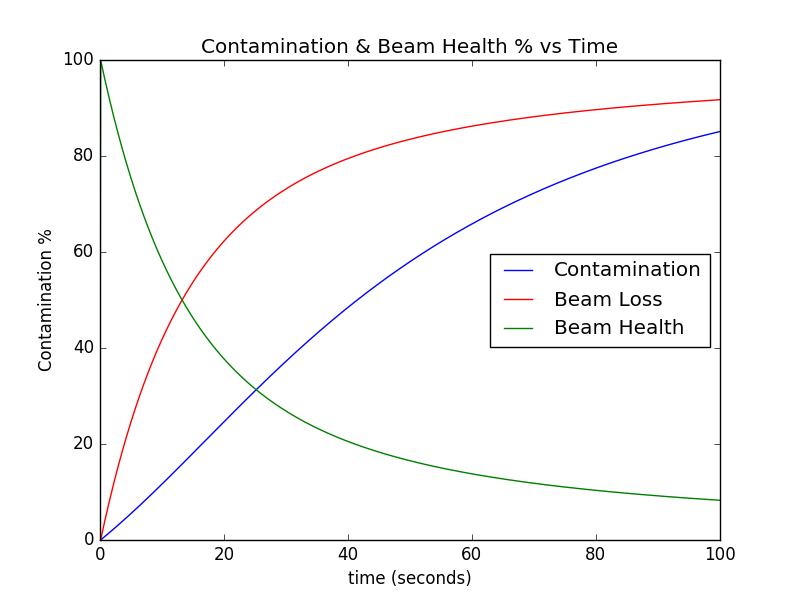
\includegraphics[width=0.5\linewidth]{./Images/Figures/figure_1-4}


\newpage
\chapter{ROOT}
\thispagestyle{fancy}

Formatting a TString can be simplified by use of the Form function.

\begin{lstlisting}
const char *someText = "Hello World!";
int someInt = 2314;

//%s corresponts to a const char*
//%d corresponds to an integer
TString output = Form("I want to say %s a total of %d times", someText, someInt);

//This will output "I want to say Hello World! a total of 2314 times"
std::cout << output;
\end{lstlisting}

\unchapter{Resources}


%Begin the backmatter.
\backmatter
{\footnotesize
\begin{thebibliography}{99}
	\bibitem{bib:Modern_Physics} Bauer, W., and Gary D. Westfall. University Physics with Modern Physics. 2nd ed. Vol. 2. New York, NY: McGraw-Hill Companies, 2014. Print. 	
	
	\bibitem{bib:Methods_Of_Theoretical}Boas, Mary L. Mathematical Methods in the Physical Sciences. 3rd ed. New York: John Wiley \& Sons, 1984. Print. 
	
	\bibitem{bib:Planets_and_telescopes} Brown, Edward, comp. ``Planets And Telescopes." (2015): n. pag. Print. Michigan State University Department of Astronomy and Physics
	
	\bibitem{bib:AST304} Brown, Edward, comp. Astronomy 304 class handouts (2015): n. pag. Print. Michigan State University Department of Astronomy and Physics
	
	\bibitem{bib:StellarAstrophysics} Brown, Edward, comp. ``Stellar Astrophysics." (2015): n. pag. Print. Michigan State University Department of Astronomy and Physics
	
	\bibitem{bib:dictionary} http://www.dictionary.com
	
	\bibitem{bib:Griffiths} Griffiths, David J. Introduction to Electrodynamics. 4th ed. N.p.: Pearson India Education Services Pvt, 2015. Print. 
	
	\bibitem{bib:PeriodicTable} Helmenstine, Todd. Periodic Table of the Elements. sciencenotes.org. 2015.
	
	\bibitem{bib:Linnemann} Linnemann, Jim, Dr. Modern Physics Lecture Notes. 2016. PHY 215 lecture notes. Department of Physics and Astronomy, Michigan State University. 
	
	\bibitem{bib:AbstractNotes} Meierfrankenfeld, Ulrich. MTH 310 Lecture Notes Based on Hungerford, Abstract Algebra. N.p.: Department of Mathematics, Michigan State U, 2015. Print. 
	
	\bibitem{electronics} Plonus, Martin. Electronics and Communications for Scientists and Engineers. San Diego: Academic, 2001. Print. 
	
	\bibitem{bib:ReitzEMTheory} Reitz, John Richard. Foundations of Electromagnetic Theory. 4th ed. N.p.: Addison-Wesley, 1992. Print. 
	
	\bibitem{bib:Kittel_ThermalPhysics}  Kittel, Charles, and Herbert Kroemer. Thermal Physics. San Francisco: W.H. Freeman, 1980. Print.
	
	\bibitem{Nazarewicz_PHY802} Nazarewicz, Witek. "MSU PHY802 Lecture Slides." Survey of Nuclear Physics 802/492 Spring 2017. Michigan State University, n.d. Web. 31 Mar. 2017. 
	
	\bibitem{bib:Foundations_Of_Astrophysics} Ryden, Barbara Sue., and Bradley M. Peterson. Foundations of Astrophysics. San Francisco: Addison-Wesley, 2010. Print. 
	
	\bibitem{bib:elementTable} ``Table of Isotopic Masses and Natural Abundances." (n.d.): n. pag. NC State University. Web. ``https://www.ncsu.edu/chemistry/msf/pdf/IsotopicMass\_NaturalAbundance.pdf". 
	
	\bibitem{bib:Classical_Mechanics} Taylor, John R. Classical Mechanics. Sausalito, CA: U Science, 2005. Print. 
	
	\bibitem{bib:WolfrmAlpha} ``Wolfram$|$Alpha: Computational Knowledge Engine." N.p., n.d. Web. 2016 x
	
	\bibitem{bib:Wolfram} ``Wolfram MathWorld: The Web's Most Extensive Mathematics Resource." Wolfram MathWorld. N.p., n.d. Web. 
	
	\bibitem{DiffEQ} Zee, Dennis G. A first Course in Differential Equations with Modeling Applications." Edition 10. Book.
\end{thebibliography}
}

\printindex

\end{document}